%
% Unless otherwise indicated, the copyright in this material is 
% owned by Joerg Evermann. This material is licensed to you under the 
% Creative Commons by-attribution non-commercial license (CC BY-NC 4.0)}
%
\section*{Learning Goals}

After reading this chapter, you should be able to:
\begin{itemize}
   \item Create and manipulate basic data structures in R, including arrays, matrices, and data frames.
   \item Create summary information from R data frames and other data structures.
   \item Use the Tidyverse packages to retrieve information from R data frames, including filtering, grouping, and aggregation of information.
   \item Use SQL to operate on R data frames to retrieve information, including filtering, grouping, and aggregation of information.
\end{itemize}


\section*{Sources and Further Reading}

The material in this chapter is based on the following sources. 

\begin{resourcebox}
Venables, W.N., Smith, D.M. and the R Core Team (2024) An Introduction to R.  \\

\footnotesize
\url{https://cran.r-project.org/doc/manuals/r-release/R-intro.pdf}\normalsize
\end{resourcebox}

This tutorial is a good, easy, and comprehensive introduction to R. It covers the most important aspects of R in 100 pages. It is continuously updated by the R team for new versions of R and new features. Chapters 1 through 7 cover the initial material in this module. 

\begin{resourcebox}
Wickham, H., Cetinkaya-Rundel, M., and Grolemund, G. (2023) R for Data Science. O'Reilly Media, Inc. \\

\footnotesize\url{https://r4ds.hadley.nz/}\normalsize
\end{resourcebox}

This is a free, open-source book directly from the authors of the popular and widely-used Tidyverse libraries. With many examples, and easy-to-understand descriptions, the book provides a solid foundation for business analytics with R. It provides sections on data import, data transformation, data visualization, and data communication, each with multiple chapters. This is a highly relevant resource for anyone doing data science in R.

\begin{resourcebox}
Posit (2024) Cheatsheet. \\

\footnotesize\url{https://posit.co/resources/cheatsheets/}\normalsize
\end{resourcebox}

Posit is the maker of the popular RStudio programming environment for R, the shiny library for building web applications and graphical dashboards with R, and a number of other open-source and proprietary tools around the R system. Posit provides a number of very helpful ''cheatsheets'' that are one-page summaries of various R libraries. The ''cheatsheets'' useful for this module is the one on the dplyr package for data transformation.


\section{Introduction}

R is a statistical software system and programming language known for its robust capabilities in data analysis, visualization, and statistical computing. It was originally developed in the early 1990s by Ross Ihaka and Robert Gentleman at the University of Auckland, New Zealand. Drawing inspiration from the S language developed at Bell Laboratories, R was designed to be a powerful and flexible tool for data analysis and statistical modeling.

One of the key advantages of R is its open-source nature, making it freely available to users worldwide. This accessibility has created a vibrant community of users and developers, continuously enhancing its functionality through comprehensive packages and extensions. The Comprehensive R Archive Network (CRAN) is a repository of these packages, offering tools for a myriad of data analysis tasks.

R's popularity stems not only from its wide range of statistical techniques, including linear and nonlinear modeling, time-series analysis, classification, clustering, and others, but also from its exceptional capabilities in data visualization. The software provides an integrated suite of tools for data manipulation, calculation, and graphical display, making it an invaluable asset for statisticians, researchers, and data scientists.

Moreover, R's programming language aspect allows for automation and customization in data analysis, which is highly beneficial for complex and repetitive tasks. Its compatibility with various data formats and integration with other programming languages and tools further enhances its versatility.

\section{Using R}

R is a command-line oriented software, that is, users type commands to perform calculations or call functions of R packages. A sequence of R commands can be assembled in a \emph{script file}, so that they may be re-run when necessary. The advantage of this type of software over one with a graphical user interface is in the repeatability and replicability of the work. Ideally, data analysts will assemble an R script file for their entire data analysis, from reading the raw data sets to the finished statistical analyses and visualizations, so that all details of the analysis are available for replication and evaluation.

\begin{figure}
\centering
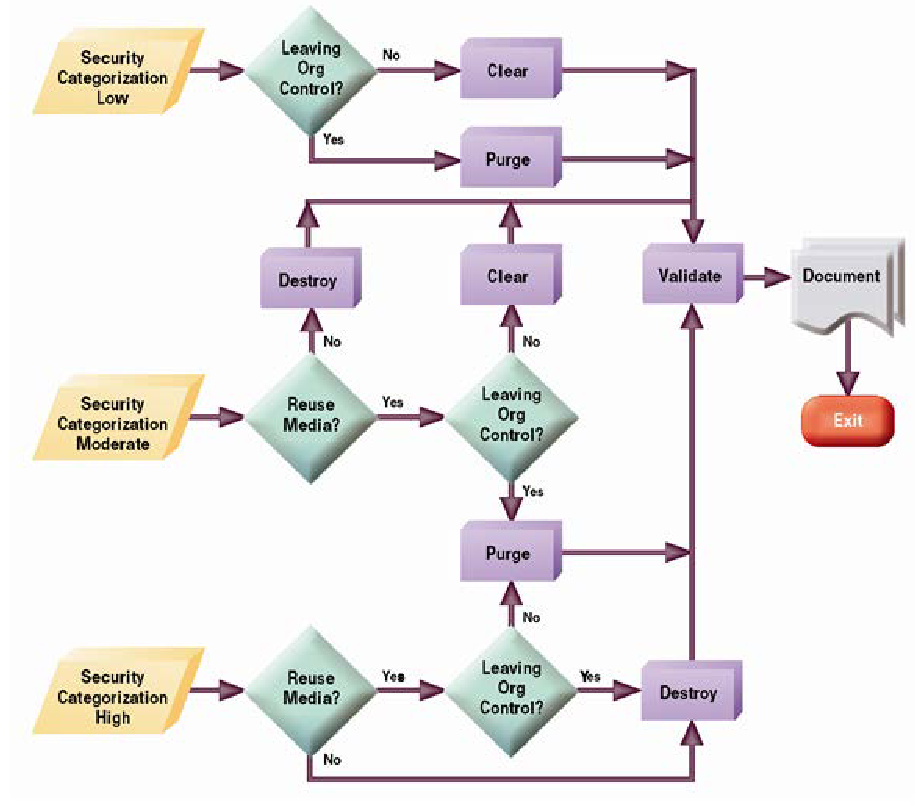
\includegraphics[width=.8\textwidth]{screen1.png}
\caption{The R command line interface}
\label{fig:r}
\end{figure}

The R system can be launched simply by invoking the \texttt{R} command from the terminal window, as shown in Figure~\ref{fig:r}. R will display its version information and prompt for command entry with a \texttt{>} prompt. 

To install R on Microsoft Windows or on MacOS, download the installation files from CRAN (Comprehensive R Archive Network) at \url{https://cran.r-project.org} and follow the instructions. R on Microsoft Windows and R on MacOS will show their command prompts inside a window but otherwise function similarly to R on Ubuntu that is installed in the course virtual machine.

\begin{infobox}
To make using R more efficient, consider doing the following:

\begin{itemize}
    \item Use the {\footnotesize\colorbox{lightgray}{up-arrow}} key to retrieve earlier commands.
    \item The \texttt{history()} function shows your command history.
    \item Use a notepad app to assemble and edit your commands easily, then copy/paste to R for execution.
    \item Use a notepad app for your results, copy/paste from R.
    \item The Ubuntu terminal uses {\footnotesize\colorbox{lightgray}{SHIFT-CTRL-X}}, {\footnotesize\colorbox{lightgray}{SHIFT-CTRL-C}}, {\footnotesize\colorbox{lightgray}{SHIFT-CTRL-V}} for cut/copy/paste.
    \item Use multiple terminal and R windows (e.g. one for executing commands, one for reading help documentation or for listing files).
    \item Don't update packages in the middle of a project.
    \item Ensure you have a \emph{repeatable, automatable script} for your entire data analysis at the end of a project.
\end{itemize}
\end{infobox}

\section{R Basics}

The most basic way to use R is to simply use it as a calculator, as shown in the following R code example. Type ''\texttt{1+1}'' at the ''\texttt{>}'' prompt, then press the \colorbox{lightgray}{RETURN} key to execute the statement. R will respond on the following line with the result:

\begin{Rcode}
> 1+1
[1] 2
\end{Rcode}

A \emph{variable} in R is a named storage space for numbers, characters, strings, and other data elements. Traditionally, values are assigned to variables using the \texttt{<-} operator, but one may also use the more ''normal'' assignment operator \texttt{=}. Using the \texttt{<-} assignment operator helps to clearly distinguish assignment from equality testing, which uses \texttt{==}. 

The following R code example introduces the R function called \texttt{print()} that does as its name suggests. Most data types and data structures that can be assigned to variables have a useful print function associated to them, so that on the interactive R command line you can simply type their name to get their value. In interactive mode, R calls the \texttt{print()} function automatically. In an R script that you execute from file, you will have to explicitly use the \texttt{print} function.

\begin{Rcode}
> a <- 3
> b <- 2
> print(a * b)
[1] 6
> a
[1] 3
\end{Rcode}

R has special symbols to denote infinity (\texttt{inf}) and results that are not a number (\texttt{NaN}):

\begin{Rcode}
> 2 / 0
[1] Inf
> 0 / 0
[1] NaN
\end{Rcode}

\noindent The boolean logical operators \emph{and} and \emph{or} are represented by the operators \texttt{\&} and \texttt{|} shown in the R code block below.

\begin{Rcode}
> TRUE & FALSE
FALSE
> TRUE | FALSE
TRUE
\end{Rcode}

\begin{infobox}
The boolean constants \texttt{TRUE} and \texttt{FALSE} can be abbreviated by \texttt{T} and \texttt{F}
\end{infobox}

Character strings in R are enclosed in single or double quotes (but not mixed quotes!). Two useful functions are \texttt{paste()} which pastes its arguments together with an optional separator between them and returns a characters string, and the \texttt{strsplit()} function which accepts a string (or vector of strings) to split, and a separator character that identifies where to split the string. It returns a list of vectors of strings.

\begin{Rcode}
> label1 = 'I Love R'
> label2 = 'and BUSI 4760'
> paste(label1, label2, sep=' ')
> strsplit('Hello World! My first string', ' ')
\end{Rcode}

Because you can assign arbitrary values to variables in R, R provides functions to test the type of the value and to coerce, that is, to change, the type of a value.

\begin{Rcode}
# Check whether it is numeric
is.numeric(2)
# Check whether it is an integer number
is.integer(3.14)
# Make it an integer
as.integer(3.14)
# Make it a character string
as.character(3.14)
# Make it a character string
as.character(TRUE)
# Make it a number
as.numeric('3.1415')
\end{Rcode}

\section{The R Environment}

The collection of variables, functions, and libraries that exists in R at any one time is called the R \emph{workspace}. The functions \texttt{ls()} and \texttt{rm()}, named after their Unix bash shell equivalents, list and remove objects from the R workspace.

\begin{Rcode}
# Show objects in workspace
> ls()
[1] "a"          "b"
# Remove one object
> rm(b)
> ls()
[1] "a"
\end{Rcode}

R comes with a built-in user manual that one can access with the \texttt{help()} function or simply the \texttt{?} operator. Help is available on any function in R, as shown in the following example. For added convenience, R provides a web browser interface to its help pages that is started by \texttt{help.start()}.

\begin{Rcode}
help()
help(lm)
?lm
??lm
help.start()
\end{Rcode}

R has a current working directory where it reads and writes files from and to. On Ubuntu Linux, this is the directory from which the \texttt{R} command was issued. R provides functions to get the working directory (\texttt{getwd()}), to set (change) it (\texttt{setwd()}, and to list the files in the working directory (\texttt{list.files()}):

\begin{Rcode}
# Get the working directory
getwd()
# Set the working directory
setwd('DataSets')
getwd()
# List files in working directory
list.files()
\end{Rcode}

\begin{infobox}It is often more convenient to change the working directory in the terminal, prior to invoking \texttt{R}.
\end{infobox}

A collection of related functions is called a \emph{library} in R. While some libraries come with the base R system, other packages will need to be downloaded and installed. The CRAN (Comrehensive R Archive Network) provides libraries in convenient form. To install packages from CRAN, use the \texttt{install.packages()} function with the name (or a vector of names) of packages to install from CRAN. Once installed, libraries can be attached to the R workspace with the \texttt{library()} function, which makes its functions and any data sets it contains available for use. 

\begin{Rcode}
# Install the tidyverse library
install.packages('tidyverse')
# Load/attach the tidyverse library
library(tidyverse)
# List all installed packages
installed.packages()
\end{Rcode}

It is sometimes useful to assemble a series of related R commands for a particular data analysis task in a script file. Script files are useful to ensure that the analysis can be repeated. The \texttt{source()} function will read and execute a file containing R commands. As noted earlier, in a script file, you will need to use the \texttt{print()} function to print the values of variables.

\begin{Rcode}
source('MyFirstScript.R')
\end{Rcode}

Finally, the \texttt{quit()} function ends an R session. When using \texttt{quit()} without arguments, R will ask whether to save the workspace image. R stores its \emph{workspace} in each directory in a file called ''.RData'' and will read it when restarted from that directory. R also stores its \emph{command history} in each directory in a file called ''.Rhsitory'' and will read it when restarted from that directory.

\begin{Rcode}
quit()
\end{Rcode}

\section{Vectors}

A common structured data type in R is a \emph{vector}\index{Vector (in R)}. A vector in R contains elements of the same data type and is ordered. When assigning elements of different datatypes to a vector, R will coerce the types of all elements to a common datatype.

\begin{Rcode}
> v <- c(1, 'a', TRUE)
> v
[1] "1"    "a"    "TRUE"
> v <- c(1, 2, 3, 4)
> v*3
[1]  3  6  9 12
\end{Rcode}

In the above example, R automatically determined that multiplication with a scalar is an element-wise operation and applies it to each element of the vector. 

Useful functions to create vectors are the sequence function \texttt{seq()}, which accepts the lower and upper limit and a step size as parameter, and the repetition function \texttt{rep()} which repeats its first argument the number of times specified by its second argument.

\begin{Rcode}
# Generate a sequence
s <- seq(0, 6, by=.5)
print(s)
# Repeat a value
r <- rep(3.5, 5)
print(r)
\end{Rcode}

R provides useful functions for numerical vectors, to find their length, their maximum and minimum value, the square root of their values, as well as the variance and standard deviation of the elements. R automatically determines whether functions are applied to the whole vector, like \texttt{var()} or \texttt{sd()}, or whether functions are applied element-wise to each element, like \texttt{sqrt()}. Vector concatenation, using the \texttt{c()} function, automatically ''flattens'' the vectors.

\begin{Rcode}
length(v)
max(v)
min(v)
sqrt(v)
var(v)
sd(v)
# Vectors get flattened
vv <- c(v, c(7, 8, 9), v)
print(vv)
\end{Rcode}

The most common way to select elements from vectors is by \emph{indexing} with a boolean vector. In the following example, the expression \texttt{vv < 5} yields a vector of boolean values (true or false). Indexing the variable \texttt{vv} with that vector determines which elements of \texttt{vv} to select (those elements for which the corresponding entry is true).

\begin{Rcode}
vv < 5
vv[vv < 5]
vv[vv < 5] <- vv[vv < 5] + 5
\end{Rcode}

Vectors can also be indexed numerically, selecting elements by their position. This is also called ''Slicing''. R allows you select a sequence of values with the \texttt{:} operator, and the exclusion of elements, or sequences of elements, using \texttt{-}. The first line in the following example selects elements at positions 3 through 7, the second line selects elemnts \emph{except} those at positions 3 through 7.

\begin{Rcode}
# Indexing is inclusive
vv[3:7]
vv[-(3:7)]
\end{Rcode}

\begin{alertbox}
\begin{itemize}
   \item R begins indexing positions with 1, while other programming languages begin at 0.
   \item Indexing in R is inclusive, that is, both the start and end index are included.
\end{itemize}
\end{alertbox}

\emph{Missing values} are designated by the special symbol \texttt{NA}. The \texttt{is.na()} function can be used to identify and select \texttt{NA} and then filter them. When an aggregation function encounters a \texttt{NA}, it will normally return a \texttt{NA}, so it is important to remove or replace \texttt{NA} values before analyzing the data. Many functions offer an option to remove \texttt{NA} values prior to applying them, as shown for the \texttt{sum()} function in the following R code block. 

\begin{Rcode}
# Introduce a missing value
v[3] <- NA
# Missing value arithmetic
v*3
# Testing for missing values
is.na(v)
# Missing values in aggregate functions
sum(v)
sum(v, na.ram=TRUE)
\end{Rcode}

Important string functions are \texttt{grep()} and \texttt{agrep()}. The \texttt{grep()} function checks whether each string in a vector of strings contains a substring that matches a regular expression, and returns the indices of strings in the vector that match the pattern. The first use of \texttt{grep()} in the following R code block matches a phone number, the second use of \texttt{grep()} matches a Canadian postal code.

\begin{Rcode}
# Match/find North American phone numbers
> grep('^([0-9]{3})[ -]?[0-9]{3}[ -]?[0-9]{4}$', 
    c('709 864 5000', 'abc def 9999', '709-865-5000'))
[1] 1 3
# Match/find Canadian postal codes
> grep('[A-V][0-9][A-V] [0-9][A-V][0-9]', 
    c('A0P 1L0', '0AB L2K', 'A0X 1Z0'))
[1] 1
\end{Rcode}

The \texttt{agrep()} function calculates the Levenshtein distance between a regular expression and a vector of strings and returns the indices of those strings that are within a certain distance. The Levenshtein distance is defined as the sum of insertions, deletions, and substitutions of characters to transform one string into another.

\begin{Rcode}
# Match/find strings up to Levenshtein distance of 3
> agrep('apple', 
    c('apricot', 'banana', 'grape', 'pineapple'), 
    max.distance=3)
[1] 1 3 4
\end{Rcode}

\section{Arrays, Matrices, and DataFrames}

R \emph{arrays}\index{Array (in R)} are multi-dimensional objects that can hold any primitive data type, usually numerical. A \emph{matrix}\index{Matrix (in R)} is simply a two-dimensional array. The following example shows how indexing (''Slicing'') generalizes from vectors to matrices and arrays simply by indexing each dimension with the same syntax as used for vectors. The \texttt{array()} function creates multi-dimensional arrays from existing data, the \texttt{dim()} function returns the number of dimensions of an array.

A few important things to note in the following R code block example:
\begin{itemize}
   \item The first dimension is the row, the second is the column
   \item Initially, the array is created from a range of numbers between 1 and 20, and the \texttt{dim} argument specifies the dimensionality. 
   \item R fills arrays by column, unless otherwise specified
   \item A dimension need not be slided or indexed, as in \texttt{a[,2]} or \texttt{a[,2:4]} which do not subset the first dimension (rows). The result is that all rows are returned in these examples. 
   \item Reversing the index reverses the result that is returned, as in \texttt{a[3:1,2:4]} which reverses the indexing of the first dimension (rows). 
\end{itemize}

\begin{Rcode}
# Default is to fill by column
a <- array(1:20, dim=c(4,5))
a
# Result:
#      [,1] [,2] [,3] [,4] [,5]
# [1,]    1    5    9   13   17
# [2,]    2    6   10   14   18
# [3,]    3    7   11   15   19
# [4,]    4    8   12   16   20
# Indexing is inclusive and starts at 1
a[,2]
a[,2:4]
a[3,2:4]
a[3:1,2:4]
\end{Rcode}

Constructing a \emph{matrix} with the \texttt{matrix()} function is similar to constructing an array, but instead of providing the dimensionality with \texttt{dim}, one must provide either the number of rows or columns (\texttt{nrow} or \texttt{ncol}) and how to fill the matrix from the elements provided using the \texttt{byrow} argument; by default, R fills arrays and matrices by column. 

The \texttt{t()} function returns the transpose of a matrix, that is, it reverses rows and columns. Binding (combining) two matrices together by columns with \texttt{cbind()} or by rows with \texttt{rbind()} requires compatible dimensions, that is, same number of rows for \texttt{cbind()} or same number of columns for \texttt{rbind()}.

\begin{Rcode}
b <- matrix(20:1, nrow=5, byrow=T)
b
# Result:
#      [,1] [,2] [,3] [,4]
# [1,]   20   19   18   17
# [2,]   16   15   14   13
# [3,]   12   11   10    9
# [4,]    8    7    6    5
# [5,]    4    3    2    1
# Test if it is a matrix
is.matrix(b)
is.matrix(a)
# Transpose
t(b)
# Bind (combine) by columns
cbind(a, t(b))
# Bind (combine) by rows
rbind(t(a), b)
\end{Rcode}

A \emph{data frame}\index{Data frame!in R} is the most widely used data structure for data analytics and statistics in R. It is essentially a table with a set of columns whose elements are of the same type. Columns are named and columns can be selected using the \texttt{\$} symbol. Useful functions on data frames are \texttt{summary()}, \texttt{head()} and \texttt{tail()}. 

The following R code block creates a variable \texttt{x} as a vector of 50 normally distributed random values using the \texttt{rnorm()} function. The variable \texttt{y} is created from vector \texttt{x} and then adds a normally distributed random variable. The two are then combined into a data frame with the \texttt{data.frame()} function. The \texttt{colnames()} function retrieves the column names, but can also change/update the column names. The \texttt{nrow()} and \texttt{ncol()} functions return the number of rows and columns, \texttt{head()} and \texttt{tail()} return the first few or last few rows, and \texttt{cov()} is an example of a statistical function that returns the covariance matrix of all columns in the data frame.

\begin{Rcode}
# Create a vector of 50 normally distributed random variables
x <- rnorm(50)
# Create another vector with random variables
y <- 2*x + rnorm(50)
# Create a data frame from the two vectors
data <- data.frame(x, y)
#  Get the column names
colnames(data)
# Update the column names
colnames(data) <- c('Pred', 'Crit')
# Get the number of rows and columns
nrow(data)
ncol(data)
# Get the "Pred" column of the data frame
data$Pred
# Print a summary
summary(data)
# Print first and last rows
head(data)
tail(data)
# Calculate the covariance matrix
cov(data)
\end{Rcode}

Data frames may be written to CSV files and read from CSV files, as shown in the following R code block. The functions \texttt{write.csv()} and \texttt{read.csv()} have a range of options for reading/writing files with or without header lines, with different separators, for skipping rows, for different decimal points, for whitespace stripping, etc. Consult the R built-in help system for details.

\begin{Rcode}
# Write CSV file into current working directory
# Omit the row names
write.csv(data, 'data.csv', row.names=FALSE)
# Read the data from the current working directory
new.data <- read.csv('data.csv')
\end{Rcode}

\begin{exercisebox}
These hands-on exercises are designed to familiarize you with the Tidyverse packages, especially the dplyr package. Use these exercises with the Pagila CSV data set.

\begin{enumerate}[nosep]
    \item Create an array with $3$ columns and $50$ rows of random numbers with mean of $2$ and standard deviation of $4$ (use the \texttt{rnorm()} function)
   \item Create a dataframe from the array and name the columns as ''A'', ''B'', ''C''
   \item ''Clip'' the values so that all values lie between $-3$ and $+7$
   \item Summarize the data
   \item Print the pairwise covariance matrix of the three columns in the data frame
   \item Find the square root of each of the diagonal entries of the covariance matrix, compare this to the standard deviation of 4. Tip: Use the \texttt{diag()} function.
   \item Save the data frame in a CSV file using your first name as file name (file ending '.csv')
\end{enumerate}
\end{exercisebox}

\section{Tidyverse}

The Tidyverse is a collection of R libraries designed for data science that share an underlying design philosophy, grammar, and data structures. Developed by Hadley Wickham and others, the Tidyverse libraries are built to work together seamlessly, making data science tasks more straightforward and intuitive. At the core of Tidyverse's philosophy is the concept of ''tidy data,'' which arranges data in a structured way that simplifies analysis. This structure involves organizing data into rows and columns where each variable is a column, each observation is a row, and each type of observational unit forms a table.

Key libraries in the Tidyverse include \emph{ggplot2} for data visualization, \emph{dplyr} for data manipulation, \emph{tidyr} for data tidying, \emph{readr} for reading data, \emph{purrr} for functional programming, and \emph{tibble} for providing a better version of a table data structure. In particular, ggplot2 allows for complex and aesthetically pleasing visualizations using a layered grammar of graphics (hence the name), while dplyr provides a set of tools for efficiently manipulating datasets, such as filtering rows, selecting columns, and aggregating data. Tidyr helps in transforming messy data into a tidy format, making it easier to analyze and visualize. Table~\ref{tab:tidyverse} contains a summary of the libraries.

\begin{table}
\centering

\renewcommand{\arraystretch}{1.25}
\begin{tabular}{l|l} \hline
dplyr & Manipulate data \\
forcats & Work with categorical variables (factors) \\
ggplot2 & Grammar of Graphics \\
lubridate & Date and time parsing and arithmetic \\
purrr & Functional programming \\
readr & Read files in various formats \\
stringr & Work with character strings \\
tibble & A tibble is better than a table \\
tidyr & Make data tidy \\ \hline
\end{tabular}
\caption{Tidyverse packages for R}
\label{tab:tidyverse}
\end{table}

Tidyverse also emphasizes readability and expressiveness in code, which not only makes data analysis easier to write but also easier to read and understand. It has become a popular choice among data scientists and statisticians for its ease of use, efficiency, and the cohesive way it handles data analysis tasks. The integration of these packages under the Tidyverse umbrella simplifies the process of data manipulation, exploration, and visualization, greatly enhancing the productivity and effectiveness of data analysis in R.

Loading and attaching the \texttt{tidyverse} library in R, using the \texttt{library(tidyverse)} function, loads all the associated core packages, as shown in Figure~\ref{fig:tidyverse}.

\begin{figure}
\centering
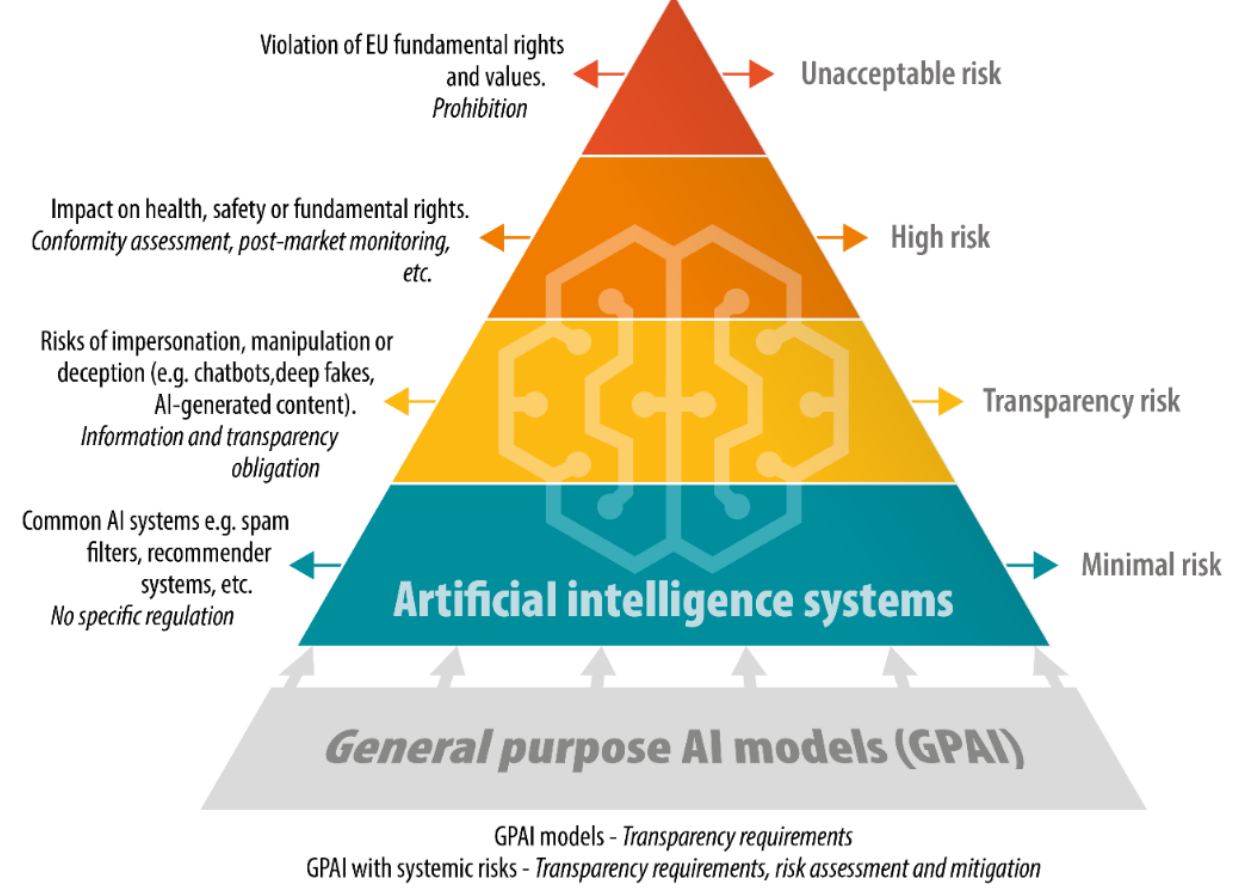
\includegraphics[width=\textwidth]{screen2.png}
\caption{Attaching the tidyverse packages in R}
\label{fig:tidyverse}
\end{figure}

\subsection*{Tidyverse Basics}

This subsection introduces basic ideas of data manipulation with the Tidyverse package, primarily using the dplyr package. A simple data set is used to illustrate basic functionality. The example dataset for this section is the Fuel Consumption Ratings for battery electric vehicles, provided the Government of Canada through its Open Government Portal\footnote{\scriptsize\url{https://open.canada.ca/data/en/dataset/98f1a129-f628-4ce4-b24d-6f16bf24dd64}}. The dataset contains the variables shown in Table~\ref{tab:fueldatachapter5}.

\begin{table}[h]
\centering
\renewcommand{\arraystretch}{1.25}

\begin{tabularx}{.9\linewidth}{|l|l|X|} \hline
  {\bf Column} & {\bf Data Type} & {\bf Definition} \\ \hline \hline
  Make & Categorical (string) & Manufacturer \\ 
  Model & Categorical (string) & Model name\\
  Year & Numeric & Model year \\
  Category & Categorical (string) & Small, Midsize, Large, Pickup, SUV, Station Wagon, etc. \\
  City & Numeric & Consumption in l/100km equiv. \\
  Hwy & Numeric & Consumption in l/100km equiv. \\
  Comb & Numeric & Consumption in l/100km equiv. \\
  Range & Numeric & Driving range in km \\ \hline
\end{tabularx}
\caption{Fuel efficiency data set variables}
\label{tab:fueldatachapter5}
\end{table}

\paragraph*{Reading Data:} When reading CSV files with readr, the data is stored in a \emph{tibble}\index{Tibble}, not a data frame. A tibble provides a number of extensions and convenience operations that make it much more capable than a data frame. When using data frames with any dplyr function, they are automatically converted to tibbles. 

The following R code reads a CSV file using the \texttt{read\_csv()} function from the Tidyverse readr library (not the \texttt{read.csv()} function from basic R!) and prints the first few lines and a summary. 

When reading CSV files with readr, the data is stored in a \emph{tibble}\index{Tibble}, not a data frame. A tibble provides a number of extensions and convenience operations that make it much more capable than a data frame. When using data frames with any dplyr function, they are automatically converted to tibbles. The output looks slightly different than that for data frames, but accomplishes essentially the same things.

\begin{Rcode}
# Read CSV into a Tibble
data <- read_csv('https://evermann.ca/busi4720/fuel.csv')
# Examine the data
# Dimensions (rows, columns)
dim(data)
# Column names
colnames(data)
# Summary
summary(data)
\end{Rcode}

The functionality in the dplyr library is intended to mirror SQL queries from the earlier module on relational databases. The main dplyr ''verbs'' used in the examples are summarized in Table~\ref{tab:dplyr}. The examples below will illustrate each of these ''verbs'' or functions and also show the equivalement SQL statements. 

\begin{table}
\centering
\renewcommand{\arraystretch}{1.25}

\begin{tabularx}{\textwidth}{l|X} \hline
\multicolumn{2}{c}{Basic} \\ \hline
\texttt{filter} & filters by row \\
\texttt{select} & selects columns to retain \\
\texttt{mutate} & creates new columns \\
\texttt{rename} & renames columns \\
\texttt{distinct} & finds unique values \\
\texttt{arrange} & sorts data rows \\
\texttt{relocate} & moves data columns \\
\texttt{group\_by} & groups data \\
\texttt{summarize} & compute aggregate information \\
\texttt{print} & prints a tibble \\  \hline
\multicolumn{2}{c}{Advanced} \\ \hline
\texttt{nest} & nests data, tibbles in tibbles \\
\texttt{full\_join} & Joins tibbles (also \texttt{outer join}, \texttt{left\_join}, \texttt{inner\_join}, \texttt{right\_join}) \\ \hline
\end{tabularx}
\caption{Important dplyr functions}
\label{tab:dplyr}
\end{table}

The tidyverse libraries make extensive use of the \emph{pipe}\index{Pipe} operator in R. The pipe operator allows chaining of function calls and plugs the result of one function as the first argument into the next function. 

\paragraph*{Filtering:} The example below starts with the tibble that was read earlier and pipes it into the \texttt{filter()} function. The filter function specifies two conditions, filtering data by vehicle Make and vehicle model Year. The output of the \texttt{filter} function is piped into the \texttt{print()} function. 

\begin{Rcode}
# Pipe a data frame or tibble into a filter and print results
data |> 
  filter(Make=='Ford', Year==2023) |> 
  print()

# Equivalent without pipe and boolean operator in filter
filter(data, Make=='Ford' & Year==2023)
\end{Rcode}

The \texttt{filter()} function is similar to the \texttt{WHERE} clause in an SQL SELECT statement and the above R code is equivalent to the following SQL statement:

\begin{sqlcode}
SELECT * 
   FROM data 
   WHERE Make=='Ford' AND Year==2023;
\end{sqlcode}

\paragraph*{Selection:} The following example adds the \texttt{select()} function to select specific columns from the data set:

\begin{Rcode}
# Pipe a data frame or tibble into a filter,
# select specific columns and print results
data |> 
  filter(Make=='Ford', Year==2023) |> 
  select(Model, Category, Range) |>
  print()
\end{Rcode}

There is no equivalent SQL clause for the \texttt{select()} function because the selection of result columns occurs in the main SELECT clause, as illustrated in the following equivalent SQL statement:

\begin{sqlcode}
SELECT Model, Category, Range 
   FROM data 
   WHERE Make=='Ford' AND Year==2023;
\end{sqlcode}

\paragraph*{Column Creation:} The next example shows the use the \texttt{mutate()} function to create a new column that expresses the range of a vehicle for highway driving. It involves a calculation using the Hwy fuel economy, the Comb combined fuel economy and the Range. The \texttt{mutate()} function is added into the above data manipulation pipeline:

\begin{Rcode}
# Pipe a data frame or tibble into a filter,
# create a new calculated column,
# select specific columns and print results
data |> 
  filter(Make=='Ford', Year==2023) |> 
  mutate(HwyRange = Range * Comb / Hwy) |>
  select(Model, Category, Range, HwyRange) |>
  print()
\end{Rcode}

An equivalent SQL statement constructs the new column in the main SELECT clause:

\begin{sqlcode}
SELECT Model, Category, Range, (Range*Comb)/Hwy AS HwyRange 
   FROM data 
   WHERE Make=='Ford' AND Year==2023;
\end{sqlcode}

\paragraph*{Renaming:} The example below shows renaming of columns using the \texttt{rename()} function. The Range column is renamed to be the CombRange column. While \texttt{mutate()} creates an additional columns, \texttt{rename()} does not and only renames an existing column. It is therefore more efficient for renaming.

\begin{Rcode}
# Pipe a data frame or tibble into a filter,
# create new calculated columns,
# rename an existing column,
# select specific columns and print results
data |> 
  filter(Make=='Ford', Year==2023) |> 
  mutate(HwyRange = Range * Comb / Hwy) |>
  mutate(CityRange = Range * Comb / City) |>
  rename(CombRange = Range) |>
  select(Model, Category, CombRange, CityRange, HwyRange) |>
  print()
\end{Rcode}

An equivalent SQL statement constructs the new column in the main SELECT clause using the AS keyword:

\begin{sqlcode}
SELECT Model, Category, 
      Range AS CombRange,
      (Range*Comb)/Hwy AS HwyRange, 
      (Range*Comb)/City As CityRange
   FROM data 
   WHERE Make=='Ford' AND Year==2023;
\end{sqlcode}

\paragraph*{Distinct Values:} The \texttt{distinct()} function can be used to find the set of unique values of a column. For example, the following R code identifies the unique vehicle Makes and Models in the data set. 

\begin{Rcode}
# Pipe a data frame or tibble into a filter,
# select distinct value combinations and print results
data |> 
  distinct(Make, Model) |>
  print()
\end{Rcode}

SQL uses the DISTINCT keyword for this purpose as well, illustrated in the following example:

\begin{sqlcode}
SELECT DISTINCT Make, Model 
  FROM data;
\end{sqlcode}

\paragraph*{Ordering:} The dplyr \texttt{arrange()} function is used to order data by values, in ascending or descending order. The following example illustrates this by adding the \texttt{arrange()} function to the data processing pipeline. The \texttt{arrange()} function orders the data first by vehicle Category in ascending order (the default ordering), then, for equal values of Model, by Range in descending order (using the \texttt{desc()} function:

\begin{Rcode}
# Pipe a data frame or tibble into a filter,
# select specific columns,
# order the data and print results
data |> 
  filter(Make=='Ford', Year==2023) |> 
  select(Model, Category, Range) |>
  arrange(Category, desc(Range)) |>
  print()
\end{Rcode}

An equivalent SQL statement uses the ORDER BY clause with the keywords ASC or DESC to indicate the direction of ordering:

\begin{sqlcode}
SELECT Model, Category, Range
   FROM data 
   WHERE Make=='Ford' AND Year==2023
   ORDER BY Category ASC, Range DESC;
\end{sqlcode}

\paragraph*{Relocating Columns:} The function \texttt{relocate()} can be used to specify the order in which columns are returned. The following code example rearranges the column order before printing by adding the \texttt{relocate()} function to the data processing pipeline:

\begin{Rcode}
# Pipe a data frame or tibble into a filter,
# select specific columns,
# order the data,
# move columns and print results
data |> 
  filter(Make=='Ford', Year==2023) |> 
  select(Model, Category, Range) |>
  arrange(Category, desc(Range)) |>
  relocate(Category, Range) |>
  print()
\end{Rcode}

SQL does not require a function or keyword in the SELECT statements. There, columns are returned in the order in which they are specified in the SELECT clause:

\begin{sqlcode}
SELECT Category, Range, Model
   FROM data 
   WHERE Make=='Ford' AND Year==2023
   ORDER BY Category ASC, Range DESC;
\end{sqlcode}

\paragraph*{Grouping and Summarizing:} The \texttt{group\_by()} function can be used to group data in preparation for computing aggregate information. It is typically used with the \texttt{summarize()} function that calculates aggregates. 

The following example shows how to compute mean fuel efficiency data, grouped by vehicle Make and vehicle Category. It adds both a \texttt{group\_by()} and a \texttt{summarize()} function into the data processing pipeline. The summarized data is then filtered again, it is sorted by vehicle Category and mean combined fuel economy, and the columns are then reordered so that vehicle Category and mean combined economy are the first two columns.

\begin{Rcode}
# Pipe a data frame or tibble into a filter,
# group the data
# summarize the data,
# filter the summary information,
# order the data,
# relocate columns and print results
data |> 
  filter(Year==2023) |> 
  group_by(Make, Category) |>
  summarize(meanCity = mean(City), 
            meanHwy = mean(Hwy),
            meanComb = mean(Comb),
            maxRange = max(Range),
            nVehicle = n()) |>
  filter(nVehicle > 1) |>
  arrange(Category, meanComb) |>
  relocate(Category, meanComb) |>
  print()
\end{Rcode}

The equivalent SQL statement also uses the GROUP BY clause. Summary information is defined in the main SELECT clause. The second \texttt{filter()} function in the R code refers to aggregate information, so that the equivalent clause in SQL is the HAVING clause:

\begin{sqlcode}
SELECT Category, 
       AVG(Comb) AS meanComb,
       Make,
       AVG(City) AS meanCity,
       AVG(Hwy) AS meanHwy,
       MAX(Range) AS maxRange,
       COUNT(*) AS nVehicle
   FROM data 
   WHERE Year==2023
   GROUP BY Make, Category
   HAVING COUNT(*) > 1
   ORDER BY Category ASC, meanComb ASC;
\end{sqlcode}

\section{Advanced Tidyverse for Data Analysis}

This section focuses on the use of dplyr to analyze data from a set of CSV files representing the data of the Pagila database. The Pagila database\footnote{\url{https://github.com/devrimgunduz/pagila}, \\
\url{https://github.com/devrimgunduz/pagila/blob/master/LICENSE.txt}} is a demonstration database originally developed for teaching and development of the MySQL RDBMS under the name Sakila\footnote{\url{https://dev.mysql.com/doc/sakila/en/}, \\
\url{https://dev.mysql.com/doc/sakila/en/sakila-license.html}}. Pagila is designed as a sample database to illustrate database concepts and is based on a fictional DVD rental store. It originally consists of several tables organized into categories like film and actor information, customer data, store inventory, and rental transactions. For this section, the Pagila data was summarized in a few related CSV files. The following R code block reads the data and coerces data types as required.

\begin{Rcode}
rentals <- read_csv('http://evermann.ca/busi4720/rentals.csv')
rentals$rating <- as.factor(rentals$rating)
rentals$language <- as.factor(rentals$language)
rentals$customer_address <- as.integer(rentals$customer_address)
rentals$customer_store <- as.integer(rentals$customer_store)
rentals$rental_staff <- as.integer(rentals$rental_staff)
rentals$payment_staff <- as.integer(rentals$payment_staff)
rentals$rental_duration <- as.integer(rentals$rental_duration)

actors <- 
  read_csv('https://evermann.ca/busi4720/actors.categories.csv')
  
addresses <- read_csv('https://evermann.ca/busi4720/addresses.csv')
addresses$phone <- as.character(addresses$phone)
\end{Rcode}

The following paragraphs show further examples of data analysis with Tidyverse and introduce additional dplyr functions or additional ways to use the dplyr functions. These example data processing pipelines mirror the example in the previous module on SQL. Only new aspects of the examples are explained.

\paragraph*{Example:} Find all films and the actors that appeared in them, ordered by film category and year, for those films that are rated PG.

\begin{Rcode}
rentals |> 
  full_join(actors, by='title', 
    suffix=c('_customer', '_actor'), 
    relationship='many-to-many') |>
  filter(rating == 'PG') |>
  mutate(actor = 
    paste(last_name_actor, ', ', first_name_actor, sep='')) |>
  rename(year=release_year) |>
  select(actor, title, category, year) |>
  distinct(actor, title, category, year) |>
  group_by(category, year, title) |> 
  nest() |>
  arrange(category, year, title) |>
  relocate(category, year, title) |>
  print(n=Inf, width=Inf)
\end{Rcode}

This R code joins the rentals data with the actors data using a full join. The join is performed on the title column that is common to both data frames/tibbles. The \texttt{suffix} argument adds distinct suffixes to column names from each data frame to avoid name clashes. The \texttt{relationship='many-to-many'} indicates the nature of the join.

The \texttt{mutate()} function creates a new column named actor, which concatenates the actor's last name and first name, separated by a comma and a space.

The data is grouped by category, year, and title, using the \texttt{group\_by()} function, and the \texttt{nest()} function is used to create a nested data frame, i.e. a data frame where the actors for each group are in a list-valued column.

\paragraph*{Example:} Find the most popular actors in the rentals in each city.

This R code block below involves combining multiple data frames and then manipulating and summarizing the data. It builds on the rental and actor tibbles from the previous example and adds address information.

\begin{Rcode}
full_data <- 
  rentals |> 
    inner_join(addresses, by=c('customer_address'='address_id')) |>
    inner_join(actors, by='title',
      suffix=c('_customer', '_actor'),
      relationship='many-to-many')
       
full_data |> 
  mutate(actor = 
    paste(last_name_actor, ', ', first_name_actor, sep='')) |>
  group_by(city, actor) |>
  summarize(count=n()) |>
  mutate(ranking = min_rank(desc(count))) |>
  filter(ranking < 4) |>
  arrange(city, ranking, actor) |>
  print(n=25)
\end{Rcode}

The analysis starts by reading a CSV file containing address information into a tibble. An inner join is performed between the rental data and the address data, matching them on a specified key in each data frame, that is, the cusomter\_address in the rentals data frame must be equal to the address\_id in the addresses data frame. 

This is followed by another inner join with the actors data frame. No join key/column is specified as the join is done on columns that have the same name in both data frames. This second join involves a many-to-many relationship and adds suffixes to to distinguish columns with the same name in the two data frames.

The data is grouped by city and actor and a new summary column is created that counts the number of occurrences (records) for each group. To create rankings, a new column is added that ranks the groups based on their count value in descending order. The \texttt{min\_rank()} function allows ties in the ranking, use \texttt{rank()} to break ties with gaps in ranking or \texttt{dense\_rank()} to break ties with no gaps in ranking. The data is then filtered to include only those records with a ranking less than 4, focusing on the top three ranks for each group.


\paragraph*{Example:} Find the customers who spend the most on rentals, with their phone numbers and cities, and the number of rentals with the higest total rental payments for each category grouped by rental duration.

\begin{Rcode}
full_data |>
   mutate(customer= paste(first_name_customer, last_name_customer)) |>
   select(customer, amount, rental_duration, category, phone, city) |>
   group_by(category, rental_duration, customer ) |>
   mutate(payments=sum(amount), num_rentals=n()) |>
   select(-amount) |>
   group_by(category, rental_duration) |>
   mutate(ranking = min_rank(desc(payments))) |>
   slice(which.min(ranking)) |>
   print(n=Inf, width=Inf)
\end{Rcode}

In this example, there is no \texttt{summarize()} function after the \texttt{group\_by()} function because \texttt{summarize()} omits all non-grouped columns, but the example requires phone numbers and cities of customers. Either these would need to be included somehow in the \texttt{summarize()} function, or, as is done in this R code, summary columns are created using the \texttt{mutate()} function instead.  Also note the ''negative'' argument to the \texttt{select()} function, which is used to remove the ''amount'' column. The data processing pipeline uses multiple \texttt{group\_by()} statements with different aggregate functions (\texttt{sum()}, \texttt{n()}, \texttt{min\_rank()}) for the different groups. Finally, the R code uses \texttt{slice()} to select the rows with the smallest ranks.

\paragraph*{Example:} Get the total rental revenue, number of rentals, and the mean and standard deviation of the rental amounts for each country.

\begin{Rcode}
full_data |>
  group_by(country) |>
  summarize(revenue=sum(amount), 
            numrentals=n(),
            mean_amount=mean(amount),
            sd_amount=sd(amount)) |>
  arrange(desc(mean_amount),
          desc(revenue)) |>
  print(n=Inf, width=Inf)  
\end{Rcode}

The R code for this query demonstrates a number different aggregate summary functions, \texttt{sum()}, \texttt{n()}, \texttt{mean()} and \texttt{sd()} (standard deviation). It also shows how to use the \texttt{desc()} function to arrange or sort data in decreasing order.

\paragraph*{Example:} Get the top 5 and the bottom 5 grossing customers for each quarter.

\begin{Rcode}
full_data |>
  mutate(customer=paste(first_name_customer,last_name_customer)) |>
  mutate(q=as.character(quarter(rental_date, with_year=T))) |>
  select(customer, q, amount, rental_date) |>
  group_by(q, customer) |>
  mutate(payments=sum(amount)) |>
  select(-amount) |>
  distinct(customer, q, payments) |>
  group_by(q) |>
  mutate(rank_top = min_rank(desc(payments))) |>
  mutate(rank_bot = min_rank(payments)) |>
  filter(rank_top <= 5 | rank_bot <= 5) |>
  arrange(q, desc(payments)) |>
  relocate(q, customer, payments, rank_top, rank_bot) |>
  print(n=Inf, width=Inf)
\end{Rcode}

The code for this query again does not use a \texttt{summarize()} function. It also shows the use of the \texttt{quarter()} function from the ''lubridate'' library. The lubridate library contains a large range of date and time related functions. Two ranking columns are created using the \texttt{mutate()} and the \texttt{min\_rank()} functions, once in descending order to get the top ranks, and again in ascending order to get the bottom ronks. The code uses \texttt{filter()} instead of \texttt{slice()} to select the top and bottom 5 ranks (using a boolean ''or'' operator), uses \texttt{arrange()} to sort the data, and then uses \texttt{relocate()} to re-arrange the order of columns prior to printing.

\paragraph*{Example:} Find the set of film titles by rental customer and the total number rentals for each customer.

\begin{Rcode}
full_data |>
  mutate(customer=paste(first_name_customer,last_name_customer)) |>
  select(customer, title) |>
  nest(titles=title) |>
  rowwise() |> 
  mutate(rentals=nrow(titles)) |>
  mutate(unique_titles=list(distinct(titles))) |>
  select(-titles) |>
  arrange(customer) |>
  print(n=Inf, width=Inf)
\end{Rcode}

The code for this query works with nested data, that is, data with columns that contain lists, created using the \texttt{nest()} function. In this example, \texttt{nest(titles=title)} creates a columns called ''titles'' that contains a list of all the elements of the ''title'' column for each customer. The R code also demonstrates row-wise operations. Both \texttt{mutate()} functions after \texttt{rowwise()} function operate by row. Specifically, the first use of the \texttt{mutate()} function creates a new column ''rentals'' which contains the number of rows in the titles column \emph{for each row} (recall that the ''titles'' column contains lists of film title). Similarly, the second use of the \texttt{mutate()} function creates a new column ''unique\_title''that contains a list of distinct film titles from the ''titles'' column \emph{for each row}.

\section{SQL and R}

The ''sqldf'' library in R allows users to perform SQL queries on R data frames. Essentially, it provides a bridge between SQL and R\index{SQL!in R}. This integration allows users who are familiar with SQL to leverage its powerful querying capabilities directly on R data structures, without the need to switch between different tools or environments.

One of the main advantages of ''sqldf'' is its ability to handle large data frames more efficiently than some of R's native functions. By utilizing SQL queries, users can perform complex data manipulations and aggregations with ease. The package supports various SQL commands including SELECT, JOIN, ORDER BY, and GROUP BY, among others, enabling a wide range of data operations that are familiar to SQL users.

Under the hood, ''sqldf'' operates by temporarily converting data frames into databases, typically by creating an in-memory SQLite database, or, alternatively, using an existing database connection to any of a variety of RDBMS such as PostgreSQL. It then creates a table for each data frame, moves the data to the database tables, and executes SQL statements. It then moves the result set back into R as a data frame. This seamless process allows for a smooth integration of SQL's data processing capabilities within the R environment.

''sqldf'' is particularly useful for R users who are already comfortable with SQL syntax and for complex data manipulation tasks that might be more cumbersome or less intuitive in R's native syntax. Its ability to handle data frames as if they were SQL tables makes it a highly valuable tool for data analysts and statisticians who work with large datasets and require the flexibility and power of SQL within the R programming environment.

The following R code block shows a very simple example. Note that the SQL \texttt{FROM} clause recognizes data frame names; any columns used in the SQL query must be named columns from those data frames.

\begin{Rcode}
library(sqldf)
result_df <- sqldf('select distinct(title) from full_data')
\end{Rcode}

When faced between the choice of data analytics using an SQL RDBMS or R/Tidyverse, there are a number of issues to consider:

\begin{itemize}
 \item \emph{Size of data}: R is limited by the amount of main memory of the computer. While large computers may offer 128GB or more, modern RDBMS can scale massively larger, in particular when distributing databases across a cluster of computers.
 \item \emph{Access speed}: RDBMS have sophisticated indexing of tables and query planners that optimize complex queries for performance. While a dplyr analysis pipeline can also be optimized by carefully considering the order of function calls, the onus is on the data analyst to do this, while an RDBMS offer this ''out-of-the-box''.
 \item \emph{Currency}: Using an RDBMS means that analytics can be performed on operational data, that is, the most current and up-to-date data. In contrast, the use of R involves first exporting data from the operational system and then analyzing it at a later time. However, while tempting, it is not generally recommended to perform complex analytics on an operational database, as it can significantly affect performance. 
 \item \emph{Transactions}: An RDBMS ensures consistent views of data across multi-user, concurrent updates. This means that, when using an operational database, the analysis sees consistent data, whereas an exported snapshot of the data may not necessarily be consistent, depending on the export mechanism.
 \item \emph{Tools}: R has tools for statistical analysis and visualization, beyond mere reporting. So far, we have considered only simple descriptive analytics. However, when the data is to be used for sophisticated statistics or predictive analytics, it is no longer possible to do this on RDBMS.
\end{itemize}

\noindent These issues motivate the following recommendations:
\begin{itemize}
 \item Do not ''hit'' operational RDBMS for heavy-weight or frequent analytics. While it may be fine to do the occasional summary analytics on an operational database, this should not be normally done. 
 \item Regularly export consistent data from RDBMS. If up-to-date data is needed, automate the export from the database to occur at regular intervals. However, note also that exporting data has a performance impact on operational databases. 
 \item Sometimes, SQL may be the more intuitive language to specify the required analysis. In these cases, use separate in-memory or on-disk RDBMS for analytics (e.g. with \texttt{sqldf}) if desired/required. 
 \item Finally, if the size of data is too large to handle in R, consider distributed tools such as Hadoop/Spark that are made for Big Data analytics.
\end{itemize}

\begin{exercisebox}

These hands-on exercises are designed to familiarize you with the Tidyverse packages, especially the dplyr package. Use these exercises with the Pagila CSV data set.

\begin{enumerate}[nosep]
  \item Find all films with a rating of 'PG'
  \item List all customers who live in Canada (with their address)
  \item Find the average \emph{actual} rental duration for all films
  \begin{itemize}
     \item This requires date arithmetic, use the \texttt{lubridate} package
  \end{itemize}
  \item Find the average overdue time for each customer
  \begin{itemize}
     \item This requires date arithmetic, use the \texttt{lubridate} package
  \end{itemize}
  \item List all films that have never been rented
  \item List the names of actors who have played in more than 15 films
\end{enumerate}
\end{exercisebox}
